\chapter{Results}
\label{c:results}

This chapter presents the experimental results across all model families, alignment
strategies, and view counts evaluated on DEX-YCB and Hi4D. Section~\ref{sec:3d_baseline}
establishes the per-frame geometric performance ceiling before any temporal alignment.
Section~\ref{sec:alignment_comparison} compares the three temporal alignment strategies.
Section~\ref{sec:sparse_view} analyses sensitivity to camera count.
Section~\ref{sec:native4d_baselines} evaluates native 4D architectures and geometry
refinement. Section~\ref{sec:opt_results} presents the Opt smoothing results.
Section~\ref{sec:qualitative} provides qualitative point cloud analysis.

\section{3D Baseline Results}
\label{sec:3d_baseline}

Table~\ref{tab:baseline_control_ggpt} reports per-frame geometric performance for all
six models and GGPT on DEX-YCB and Hi4D, averaged over two-, three-, and four-view
configurations. These per-frame aligned results serve as the geometric ceiling: no
temporal alignment or smoothing has been applied, and each frame is registered
independently to its ground-truth counterpart.

\begin{table}[t]
\centering
\scriptsize
\setlength{\tabcolsep}{4pt}
\begin{tabular}{lllccc}
\toprule
Dataset & Model Family & Method & Chamfer $\downarrow$ & Accuracy (Stat/Dyn) $\uparrow$ & Completeness (Stat/Dyn) $\uparrow$ \\
\midrule
\multirow{12}{*}{Dex-YCB} & MAST3R-SfM & Baseline & \underline{0.025} & 73.5 / 71.3 & 65.5 / \underline{62.4} \\
 & MAST3R-SfM & GGPT & 0.167 & 52.5 / 45.2 & 53.1 / 49.7 \\
\cmidrule(l){2-6}
 & VGGT & Baseline & \underline{0.025} & 80.7 / 69.8 & 61.7 / \textbf{62.6} \\
 & VGGT & GGPT & 0.203 & 59.5 / 60.4 & 52.2 / 47.6 \\
\cmidrule(l){2-6}
 & PI3 & Baseline & \textbf{0.022} & \textbf{94.4} / \underline{77.3} & \underline{80.6} / 58.6 \\
 & PI3 & GGPT & 0.105 & 74.4 / 30.7 & 66.2 / 40.7 \\
\cmidrule(l){2-6}
 & PI3X & Baseline & 0.028 & \underline{92.1} / \textbf{81.4} & 77.7 / 60.6 \\
 & PI3X & GGPT & 0.107 & 85.7 / 46.4 & \textbf{80.9} / 55.9 \\
\cmidrule(l){2-6}
 & VGGT4D & Baseline & 0.053 & 57.9 / 53.8 & 41.6 / 45.6 \\
 & VGGT4D & GGPT & 0.239 & 42.3 / 52.3 & 25.4 / 46.2 \\
\cmidrule(l){2-6}
 & MonoFusion & Baseline & 0.050 & 40.4 / 28.5 & 46.0 / 34.1 \\
 & MonoFusion & GGPT & 0.082 & 9.4 / 12.6 & 6.6 / 8.1 \\
\midrule
\multirow{11}{*}{Hi4D} & MAST3R-SfM & Baseline & 0.158 & -- / 7.7 & -- / 8.8 \\
 & MAST3R-SfM & GGPT & 0.786 & -- / 1.8 & -- / 2.1 \\
\cmidrule(l){2-6}
 & VGGT & Baseline & 0.095 & -- / \underline{13.8} & -- / 10.3 \\
 & VGGT & GGPT & 1.510 & -- / 2.2 & -- / 2.5 \\
\cmidrule(l){2-6}
 & PI3 & Baseline & \textbf{0.072} & -- / \textbf{14.4} & -- / \textbf{16.7} \\
 & PI3 & GGPT & 0.447 & -- / 2.6 & -- / 3.7 \\
\cmidrule(l){2-6}
 & PI3X & Baseline & \underline{0.078} & -- / 13.5 & -- / \underline{15.4} \\
 & PI3X & GGPT & 0.396 & -- / 2.5 & -- / 4.0 \\
\cmidrule(l){2-6}
 & VGGT4D & Baseline & 0.230 & -- / 8.5 & -- / 8.2 \\
 & VGGT4D & GGPT & 1.057 & -- / 1.6 & -- / 1.8 \\
\cmidrule(l){2-6}
 & MonoFusion & Baseline & 0.356 & -- / 4.5 & -- / 2.7 \\
\bottomrule
\end{tabular}
\caption{Per-frame geometric performance averaged over 2, 3, and 4 views on DEX-YCB
and Hi4D. Each frame is aligned independently to ground truth; no temporal alignment
is applied. Accuracy and completeness are reported as percentages at a 1\,cm threshold.
Static/dynamic decomposition is reported for DEX-YCB only; Hi4D provides no static
background so all evaluated points are dynamic. GGPT post-processes Strategy-2 aligned
output for spatial models and native output for VGGT4D and MonoFusion.
\textbf{Bold} = best per column within dataset, \underline{underline} = second best.}
\label{tab:baseline_control_ggpt}
\end{table}

On DEX-YCB, PI3 achieves the lowest Chamfer distance (0.022\,m) and the highest static
accuracy (94.4\,\%), establishing it as the strongest spatial estimator at the 1\,cm
robotics threshold. PI3X leads on dynamic accuracy (81.4\,\%), though its baseline
Chamfer of 0.028\,m is slightly higher than PI3. MASt3R-SfM and VGGT tie on Chamfer at
0.025\,m; VGGT achieves higher static accuracy (80.7\,\% vs.\ 73.5\,\%). The four
spatial models consistently outperform both native 4D architectures: VGGT4D reaches
0.053\,m Chamfer with 57.9\,\% static accuracy, and MonoFusion 0.050\,m with 40.4\,\%
static accuracy. GGPT worsens Chamfer for every backbone without exception, a result
discussed in detail in Section~\ref{sec:native4d_baselines}.

On Hi4D, the model ordering is consistent with DEX-YCB. PI3 achieves the lowest Chamfer
(0.072\,m) and highest dynamic accuracy (14.4\,\%) and completeness (16.7\,\%), with
PI3X following closely (0.078\,m, 13.5\,\%). Dynamic accuracy values on Hi4D are
substantially lower than on DEX-YCB across all models, reflecting the greater difficulty
of close human--human interaction sequences with stronger self-occlusions and larger
non-rigid motion. VGGT4D (0.230\,m) and MonoFusion (0.356\,m) degrade more severely
than spatial models on this out-of-distribution dataset. Static accuracy and completeness
are not reported for Hi4D, since the background is masked during preprocessing and all
evaluated points belong to dynamic subject regions (Section~\ref{sec:datasets}).



\section{Alignment strategy comparison}
\label{sec:alignment_comparison}

Lifting per-frame reconstructions into a temporally coherent 4D representation requires
bringing independently reconstructed frames into a shared coordinate system. The three
strategies introduced in Section~\ref{sec:alignment_strategies} differ in how they
establish this shared system, and consequently in how much geometric distortion they
introduce. Table~\ref{tab:strategy_extended} compares all three on DEX-YCB and Hi4D,
reporting Chamfer distance, $\Delta_{\text{consistency}}$, and camera pose metrics
pooled over view counts. $\Delta_{\text{consistency}}$ isolates the geometric cost of
the alignment itself: it measures the difference between the sequence-level Chamfer
distance after temporal alignment and the per-frame Chamfer distance under independent
ground-truth registration (Section~\ref{sec:metrics}). Camera pose metrics serve as an
additional indicator of alignment quality, since the same Umeyama transformations
estimated for the point clouds are applied to the cameras.

\begin{table*}[t]
\centering
\scriptsize
\setlength{\tabcolsep}{4pt}
\begin{tabular}{lllccccc}
\toprule
Dataset & Model Family & Method & Chamfer $\downarrow$ & $\Delta$Cons. $\downarrow$ & ATE $\downarrow$ & RPE $\downarrow$ & Rot Err $\downarrow$ \\
\midrule
\multirow{24}{*}{Dex-YCB} & \multirow{6}{*}{MAST3R-SfM} & Strategy 1 & 0.032 $\pm$ 0.009 & 0.007 $\pm$ 0.001 & 0.129 & 0.073 & 2.210 \\
 &  & Strategy 2 & 0.031 $\pm$ 0.011 & 0.006 $\pm$ 0.003 & 0.127 & 0.071 & \textbf{2.064} \\
 &  & Strategy 3 & \textbf{0.031} $\pm$ 0.010 & \textbf{0.005} $\pm$ 0.001 & \textbf{0.124} & \textbf{0.067} & 2.068 \\
\cmidrule(l){4-8}
 &  & GGPT (S1) & \textbf{0.167} $\pm$ 0.057 & 0.007 $\pm$ 0.001 & 0.120 & 0.069 & 2.220 \\
 &  & GGPT (S2) & \textbf{0.167} $\pm$ 0.057 & 0.006 $\pm$ 0.002 & 0.121 & 0.071 & 2.216 \\
 &  & GGPT (S3) & 0.167 $\pm$ 0.058 & \textbf{0.006} $\pm$ 0.001 & \textbf{0.119} & \textbf{0.067} & \textbf{2.182} \\
\cmidrule(l){2-8}
 & \multirow{6}{*}{VGGT} & Strategy 1 & 0.032 $\pm$ 0.003 & 0.007 $\pm$ 0.002 & 0.345 & 0.084 & 2.487 \\
 &  & Strategy 2 & \textbf{0.030} $\pm$ 0.004 & \textbf{0.005} $\pm$ 0.002 & 0.337 & \textbf{0.081} & 2.378 \\
 &  & Strategy 3 & 0.031 $\pm$ 0.002 & 0.006 $\pm$ 0.002 & \textbf{0.336} & 0.081 & \textbf{2.314} \\
\cmidrule(l){4-8}
 &  & GGPT (S1) & 0.203 $\pm$ 0.021 & \textbf{0.006} $\pm$ 0.001 & 0.356 & \textbf{0.088} & 2.583 \\
 &  & GGPT (S2) & 0.203 $\pm$ 0.021 & \textbf{0.006} $\pm$ 0.001 & 0.354 & 0.088 & 2.695 \\
 &  & GGPT (S3) & \textbf{0.202} $\pm$ 0.021 & 0.006 $\pm$ 0.002 & \textbf{0.353} & \textbf{0.088} & \textbf{2.506} \\
\cmidrule(l){2-8}
 & \multirow{6}{*}{PI3} & Strategy 1 & \textbf{0.030} $\pm$ 0.004 & 0.008 $\pm$ 0.003 & 0.078 & 0.073 & 1.562 \\
 &  & Strategy 2 & 0.031 $\pm$ 0.004 & 0.008 $\pm$ 0.005 & 0.079 & 0.073 & 1.543 \\
 &  & Strategy 3 & 0.030 $\pm$ 0.005 & \textbf{0.007} $\pm$ 0.003 & \textbf{0.074} & \textbf{0.068} & \textbf{1.491} \\
\cmidrule(l){4-8}
 &  & GGPT (S1) & 0.106 $\pm$ 0.033 & \textbf{0.010} $\pm$ 0.006 & 0.085 & 0.070 & 1.966 \\
 &  & GGPT (S2) & \textbf{0.105} $\pm$ 0.032 & \textbf{0.010} $\pm$ 0.006 & 0.087 & 0.073 & \textbf{1.866} \\
 &  & GGPT (S3) & 0.105 $\pm$ 0.033 & \textbf{0.010} $\pm$ 0.006 & \textbf{0.084} & \textbf{0.069} & 1.961 \\
\cmidrule(l){2-8}
 & \multirow{6}{*}{PI3X} & Strategy 1 & 0.031 $\pm$ 0.003 & 0.003 $\pm$ 0.003 & 0.067 & \textbf{0.050} & 1.678 \\
 &  & Strategy 2 & \textbf{0.030} $\pm$ 0.003 & 0.003 $\pm$ 0.003 & 0.066 & \textbf{0.050} & \textbf{1.640} \\
 &  & Strategy 3 & 0.030 $\pm$ 0.004 & \textbf{0.002} $\pm$ 0.002 & \textbf{0.066} & \textbf{0.050} & 1.642 \\
\cmidrule(l){4-8}
 &  & GGPT (S1) & \textbf{0.107} $\pm$ 0.037 & \textbf{0.002} $\pm$ 0.001 & 0.073 & 0.054 & 1.649 \\
 &  & GGPT (S2) & \textbf{0.107} $\pm$ 0.037 & \textbf{0.002} $\pm$ 0.001 & 0.076 & 0.056 & 1.661 \\
 &  & GGPT (S3) & \textbf{0.107} $\pm$ 0.037 & \textbf{0.002} $\pm$ 0.001 & \textbf{0.072} & \textbf{0.054} & \textbf{1.643} \\
\midrule
\multirow{24}{*}{Hi4D} & \multirow{6}{*}{MAST3R-SfM} & Strategy 1 & \textbf{0.279} $\pm$ 0.016 & \textbf{0.121} $\pm$ 0.007 & \textbf{2.014} & \textbf{2.140} & 32.369 \\
 &  & Strategy 2 & 0.302 $\pm$ 0.026 & 0.144 $\pm$ 0.017 & 2.069 & 2.189 & 32.450 \\
 &  & Strategy 3 & 0.330 $\pm$ 0.023 & 0.172 $\pm$ 0.015 & 2.114 & 2.190 & \textbf{29.855} \\
\cmidrule(l){4-8}
 &  & GGPT (S1) & 0.799 $\pm$ 0.093 & -0.013 $\pm$ 0.008 & 1.831 & 1.942 & 28.639 \\
 &  & GGPT (S2) & 0.795 $\pm$ 0.096 & -0.017 $\pm$ 0.007 & 1.848 & \textbf{1.927} & 28.427 \\
 &  & GGPT (S3) & \textbf{0.764} $\pm$ 0.080 & \textbf{-0.048} $\pm$ 0.022 & \textbf{1.804} & 1.939 & \textbf{27.930} \\
\cmidrule(l){2-8}
 & \multirow{6}{*}{VGGT} & Strategy 1 & \textbf{0.099} $\pm$ 0.010 & 0.004 $\pm$ 0.002 & 8.088 & 0.365 & 5.332 \\
 &  & Strategy 2 & \textbf{0.099} $\pm$ 0.010 & \textbf{0.004} $\pm$ 0.001 & 8.094 & 0.364 & \textbf{5.157} \\
 &  & Strategy 3 & 0.107 $\pm$ 0.016 & 0.012 $\pm$ 0.007 & \textbf{7.882} & \textbf{0.351} & 5.212 \\
\cmidrule(l){4-8}
 &  & GGPT (S1) & 1.528 $\pm$ 0.069 & -0.023 $\pm$ 0.019 & 8.085 & 0.899 & 18.309 \\
 &  & GGPT (S2) & 1.531 $\pm$ 0.066 & -0.020 $\pm$ 0.009 & 8.129 & \textbf{0.874} & \textbf{17.686} \\
 &  & GGPT (S3) & \textbf{1.473} $\pm$ 0.108 & \textbf{-0.078} $\pm$ 0.078 & \textbf{7.548} & 0.889 & 17.897 \\
\cmidrule(l){2-8}
 & \multirow{6}{*}{PI3} & Strategy 1 & \textbf{0.075} $\pm$ 0.007 & \textbf{0.003} $\pm$ 0.001 & \textbf{1.864} & \textbf{0.298} & \textbf{2.488} \\
 &  & Strategy 2 & \textbf{0.075} $\pm$ 0.007 & \textbf{0.003} $\pm$ 0.001 & \textbf{1.864} & \textbf{0.298} & \textbf{2.488} \\
 &  & Strategy 3 & \textbf{0.075} $\pm$ 0.007 & \textbf{0.003} $\pm$ 0.001 & \textbf{1.864} & \textbf{0.298} & \textbf{2.488} \\
\cmidrule(l){4-8}
 &  & GGPT (S1) & \textbf{0.445} $\pm$ 0.011 & \textbf{0.003} $\pm$ 0.002 & 2.076 & 0.821 & 16.925 \\
 &  & GGPT (S2) & 0.447 $\pm$ 0.012 & 0.004 $\pm$ 0.001 & 2.070 & \textbf{0.796} & \textbf{16.373} \\
 &  & GGPT (S3) & 0.449 $\pm$ 0.008 & 0.006 $\pm$ 0.005 & \textbf{2.052} & 0.811 & 16.613 \\
\cmidrule(l){2-8}
 & \multirow{6}{*}{PI3X} & Strategy 1 & \textbf{0.088} $\pm$ 0.007 & \textbf{0.010} $\pm$ 0.004 & \textbf{1.470} & \textbf{1.543} & \textbf{6.625} \\
 &  & Strategy 2 & \textbf{0.088} $\pm$ 0.007 & \textbf{0.010} $\pm$ 0.004 & \textbf{1.470} & \textbf{1.543} & \textbf{6.625} \\
 &  & Strategy 3 & \textbf{0.088} $\pm$ 0.007 & \textbf{0.010} $\pm$ 0.004 & \textbf{1.470} & \textbf{1.543} & \textbf{6.625} \\
\cmidrule(l){4-8}
 &  & GGPT (S1) & 0.397 $\pm$ 0.016 & 0.003 $\pm$ 0.003 & 1.791 & 1.930 & 18.633 \\
 &  & GGPT (S2) & 0.396 $\pm$ 0.016 & \textbf{0.002} $\pm$ 0.002 & 1.786 & 1.921 & \textbf{18.189} \\
 &  & GGPT (S3) & \textbf{0.396} $\pm$ 0.015 & 0.002 $\pm$ 0.003 & \textbf{1.774} & \textbf{1.917} & 18.318 \\
\bottomrule
\end{tabular}
\caption{Alignment strategy comparison on DEX-YCB and Hi4D, pooled over view counts.
All metrics are averaged over subjects and view counts. Chamfer and
$\Delta_{\text{consistency}}$ are reported as mean $\pm$ std over subjects.
$\Delta_{\text{consistency}}$ measures the increase in Chamfer distance introduced by
temporal alignment relative to independent per-frame ground-truth registration; a value
near zero indicates that alignment preserves per-frame geometry faithfully. ATE, RPE,
and rotation error are averaged over views and serve as additional indicators of
alignment quality, since the same transformations computed for the point clouds are
applied to the cameras. \textbf{Bold} = best within each strategy block or GGPT block.}
\label{tab:strategy_extended}
\end{table*}

On DEX-YCB, the three strategies produce closely matched Chamfer distances across all
models, with differences of at most 0.001\,m. Strategy 3 achieves the lowest
$\Delta_{\text{consistency}}$ in most cases and the best camera pose metrics, indicating
that pose-graph optimisation over all $\mathcal{O}(T^2)$ pairwise edges introduces less
geometric distortion than single-path strategies. For MASt3R-SfM, Strategy 3 reduces
$\Delta_{\text{consistency}}$ from 0.007 (Strategy 1) to 0.005 and achieves the best
ATE (0.124) and RPE (0.067). For VGGT, Strategy 2 produces the lowest Chamfer (0.030\,m)
and $\Delta_{\text{consistency}}$ (0.005). No single strategy dominates across all
models and metrics; the differences are modest throughout. Strategy 2 is selected as
the alignment basis for the temporal smoothing refinement in
Section~\ref{sec:opt_results}, with the rationale for this choice discussed in
Chapter~\ref{c:discussion}.

On Hi4D, the alignment strategies are applied directly to the dynamic scene points,
since no static background is available after preprocessing (Section~\ref{sec:datasets}).
The strategies were designed to exploit static correspondences as stable anchors for
temporal registration; applying them to dynamic content instead is an approximation that
relies on inter-frame motion being sufficiently small for the alignments to remain
meaningful. For MASt3R-SfM, the results show a clear degradation with more complex
strategies: Chamfer increases from 0.279\,m under Strategy 1 to 0.302\,m under
Strategy 2 and 0.330\,m under Strategy 3, with $\Delta_{\text{consistency}}$ rising
correspondingly from 0.121 to 0.172. For VGGT, Strategy 1 and Strategy 2 produce
identical Chamfer (0.099\,m), with Strategy 3 increasing to 0.107\,m. For PI3 and PI3X,
all three strategies produce identical results across every metric. The static
correspondence signal that drives differentiation between the strategies is absent on
Hi4D, and the dynamic points provide insufficient variation for the alignment to produce
different outcomes across strategy variants. Hi4D results are therefore reported for
completeness but reflect the performance of the underlying models rather than the
properties of the alignment strategies.

\section{Sparse-View Sensitivity}
\label{sec:sparse_view}

The camera configurations of Section~\ref{sec:datasets} span two, three, and four
views, progressively increasing multi-view coverage. This section isolates the effect
of camera count on reconstruction quality by comparing Strategy-2 aligned outputs
across all six models. Table~\ref{tab:global_performance_dex_ycb} reports the full
per-view-count breakdown on DEX-YCB, covering geometric fidelity, static/dynamic
decomposition, and temporal stability at each level of sparsity. Opt and GGPT results
are included in the table for reference; their detailed analysis follows in
Sections~\ref{sec:native4d_baselines} and~\ref{sec:opt_results}.

\begin{table*}[t]
\centering
\scriptsize
\setlength{\tabcolsep}{3pt}
\begin{tabular}{cllcccccc}
\toprule
View Count & Model Family & Method/Pipeline & Chamfer $\downarrow$ & Accuracy (Stat/Dyn) $\uparrow$ & Completeness (Stat/Dyn) $\uparrow$ & Jitter Mean $\downarrow$ & HF Jitter $\downarrow$ & Drift Mean $\downarrow$ \\
\midrule
\multirow{16}{*}{2} & MAST3R-SfM & Strategy-2 & 0.043 & 0.463 / 0.406 & 0.364 / 0.336 & 0.011 & 0.019 & 0.033 \\
 &  & +opt (ours) & 0.046 & 0.404 / 0.348 & 0.319 / 0.303 & \textbf{0.001} & \textbf{0.000} & 0.023 \\
 &  & GGPT (S2) & 0.230 & 0.535 / 0.391 & 0.507 / 0.433 & 0.008 & 0.014 & 0.029 \\
 & VGGT & Strategy-2 & 0.034 & 0.642 / 0.501 & 0.439 / 0.485 & 0.009 & 0.015 & 0.060 \\
 &  & +opt (ours) & 0.039 & 0.635 / 0.481 & 0.447 / 0.490 & 0.003 & \textbf{0.000} & 0.054 \\
 &  & GGPT (S2) & 0.201 & 0.570 / \textbf{0.611} & 0.540 / 0.482 & 0.007 & 0.011 & 0.032 \\
 & PI3 & Strategy-2 & 0.031 & 0.712 / 0.435 & 0.622 / 0.283 & 0.006 & 0.010 & 0.007 \\
 &  & +opt (ours) & \textbf{0.026} & 0.767 / 0.497 & 0.675 / 0.438 & \underline{0.002} & \textbf{0.000} & 0.034 \\
 &  & GGPT (S2) & 0.072 & \textbf{0.811} / 0.306 & \textbf{0.755} / \underline{0.513} & 0.004 & 0.006 & 0.016 \\
 & PI3X & Strategy-2 & \underline{0.027} & 0.753 / \underline{0.593} & 0.660 / 0.481 & 0.005 & 0.008 & 0.035 \\
 &  & +opt (ours) & 0.040 & 0.694 / 0.442 & 0.616 / 0.390 & \underline{0.002} & \textbf{0.000} & 0.034 \\
 &  & GGPT (S2) & 0.065 & \underline{0.789} / 0.353 & \underline{0.724} / \textbf{0.572} & 0.003 & 0.006 & 0.015 \\
 & VGGT4D & Native 4D & 0.051 & 0.371 / 0.385 & 0.371 / 0.403 & 0.003 & 0.005 & 0.010 \\
 &  & GGPT (N4D) & 0.213 & 0.345 / 0.346 & 0.317 / 0.404 & 0.004 & 0.006 & 0.014 \\
 & MonoFusion & Native 4D & 0.081 & 0.155 / 0.115 & 0.199 / 0.145 & \textbf{0.001} & \underline{0.001} & \underline{0.001} \\
 &  & GGPT (N4D) & 0.091 & 0.111 / 0.152 & 0.101 / 0.093 & \underline{0.002} & 0.003 & \textbf{0.000} \\
\midrule
\multirow{16}{*}{3} & MAST3R-SfM & Strategy-2 & \underline{0.023} & 0.738 / 0.617 & 0.663 / 0.522 & 0.007 & 0.011 & 0.020 \\
 &  & +opt (ours) & \textbf{0.022} & 0.755 / 0.627 & 0.683 / 0.542 & \textbf{0.001} & \textbf{0.000} & 0.015 \\
 &  & GGPT (S2) & 0.119 & 0.534 / 0.487 & 0.576 / 0.534 & 0.006 & 0.011 & 0.020 \\
 & VGGT & Strategy-2 & 0.028 & 0.731 / 0.608 & 0.610 / 0.508 & 0.005 & 0.009 & 0.028 \\
 &  & +opt (ours) & 0.028 & 0.731 / 0.597 & 0.622 / 0.510 & \textbf{0.001} & \textbf{0.000} & 0.022 \\
 &  & GGPT (S2) & 0.224 & 0.602 / 0.557 & 0.549 / 0.451 & 0.004 & 0.007 & 0.022 \\
 & PI3 & Strategy-2 & 0.035 & \underline{0.897} / 0.675 & 0.693 / 0.383 & 0.006 & 0.011 & 0.048 \\
 &  & +opt (ours) & 0.033 & 0.873 / \underline{0.682} & 0.698 / \underline{0.586} & \textbf{0.001} & \textbf{0.000} & 0.022 \\
 &  & GGPT (S2) & 0.136 & 0.711 / 0.218 & 0.664 / 0.294 & 0.004 & 0.006 & 0.020 \\
 & PI3X & Strategy-2 & 0.032 & \textbf{0.909} / \textbf{0.720} & \underline{0.757} / 0.490 & 0.005 & 0.008 & 0.011 \\
 &  & +opt (ours) & 0.036 & 0.852 / 0.658 & 0.721 / 0.447 & \textbf{0.001} & \textbf{0.000} & 0.020 \\
 &  & GGPT (S2) & 0.137 & 0.854 / 0.503 & \textbf{0.866} / 0.508 & \underline{0.003} & 0.005 & 0.008 \\
 & VGGT4D & Native 4D & 0.041 & 0.625 / 0.530 & 0.529 / 0.525 & \underline{0.003} & 0.005 & 0.010 \\
 &  & GGPT (N4D) & 0.184 & 0.469 / 0.587 & 0.336 / \textbf{0.614} & \underline{0.003} & 0.004 & 0.008 \\
 & MonoFusion & Native 4D & 0.031 & 0.544 / 0.390 & 0.641 / 0.435 & \textbf{0.001} & \underline{0.001} & \textbf{0.001} \\
 &  & GGPT (N4D) & 0.091 & 0.046 / 0.082 & 0.040 / 0.048 & \underline{0.003} & 0.005 & \underline{0.005} \\
\midrule
\multirow{16}{*}{4} & MAST3R-SfM & Strategy-2 & \underline{0.026} & 0.693 / 0.657 & 0.609 / 0.576 & 0.009 & 0.015 & 0.034 \\
 &  & +opt (ours) & \underline{0.026} & 0.705 / 0.665 & 0.621 / 0.594 & \textbf{0.001} & \textbf{0.000} & 0.026 \\
 &  & GGPT (S2) & 0.152 & 0.507 / 0.479 & 0.514 / 0.523 & 0.008 & 0.014 & 0.033 \\
 & VGGT & Strategy-2 & 0.027 & 0.741 / 0.656 & 0.567 / 0.556 & 0.005 & 0.008 & 0.021 \\
 &  & +opt (ours) & 0.029 & 0.727 / 0.645 & 0.578 / 0.562 & \textbf{0.001} & \textbf{0.000} & 0.019 \\
 &  & GGPT (S2) & 0.183 & 0.595 / 0.654 & 0.473 / 0.500 & 0.004 & 0.007 & 0.018 \\
 & PI3 & Strategy-2 & \underline{0.026} & 0.870 / 0.719 & 0.704 / 0.552 & 0.006 & 0.009 & 0.018 \\
 &  & +opt (ours) & \textbf{0.025} & 0.863 / 0.750 & 0.739 / \textbf{0.678} & \textbf{0.001} & \textbf{0.000} & 0.020 \\
 &  & GGPT (S2) & 0.108 & 0.728 / 0.406 & 0.586 / 0.419 & 0.006 & 0.009 & 0.027 \\
 & PI3X & Strategy-2 & 0.032 & \textbf{0.943} / \textbf{0.885} & \underline{0.761} / \underline{0.660} & 0.005 & 0.009 & 0.019 \\
 &  & +opt (ours) & 0.035 & 0.912 / \underline{0.836} & 0.759 / 0.629 & \textbf{0.001} & \textbf{0.000} & 0.014 \\
 &  & GGPT (S2) & 0.118 & \underline{0.927} / 0.545 & \textbf{0.834} / 0.591 & 0.007 & 0.012 & 0.011 \\
 & VGGT4D & Native 4D & 0.069 & 0.691 / 0.628 & 0.305 / 0.388 & \underline{0.003} & 0.006 & 0.007 \\
 &  & GGPT (N4D) & 0.321 & 0.455 / 0.636 & 0.108 / 0.369 & 0.004 & 0.007 & 0.022 \\
 & MonoFusion & Native 4D & 0.031 & 0.620 / 0.470 & 0.634 / 0.512 & \textbf{0.001} & \underline{0.001} & \underline{0.001} \\
 &  & GGPT (N4D) & 0.064 & 0.125 / 0.143 & 0.058 / 0.102 & \textbf{0.001} & \underline{0.001} & \textbf{0.000} \\
\bottomrule
\end{tabular}
\caption{Per-view-count spatio-temporal performance on DEX-YCB. Each block reports
results for a fixed number of input views (2, 3, or 4). Chamfer distance is in metres.
Accuracy and completeness are evaluated at a 1\,cm threshold and decomposed into
static and dynamic scene regions; values range from 0 (no surface recovered within
threshold) to 1 (all surface recovered). Temporal metrics---jitter mean,
high-frequency (HF) jitter, and drift---are computed on static scene anchors and
reported in metres. Strategy-2 serves as the unsmoothed temporal alignment baseline
for spatial models. +Opt applies the proposed Gaussian-weighted temporal smoothing.
GGPT\,(S2) and GGPT\,(N4D) apply geometry-grounded point transformer refinement to
Strategy-2 and native 4D model outputs, respectively.
\textbf{Bold} = best per column within each view-count block,
\underline{underline} = second best.}
\label{tab:global_performance_dex_ycb}
\end{table*}

Spatial models show consistent improvement with additional views on DEX-YCB. PI3's
Chamfer distance decreases from 0.031\,m at two views to 0.026\,m at four views, with
static accuracy rising from 71.2\,\% to 87.0\,\%. PI3X exhibits the strongest gains in
dynamic reconstruction: dynamic accuracy improves from 59.3\,\% at two views to
88.5\,\% at four views, while static accuracy reaches 94.3\,\%---the highest value
across all models and view counts. MASt3R-SfM benefits most from the addition of a
third camera, where Chamfer drops from 0.043\,m to 0.023\,m and static accuracy
increases from 46.3\,\% to 73.8\,\%; four-view Chamfer remains competitive at
0.026\,m. VGGT improves monotonically, with Chamfer decreasing from 0.034\,m at two
views to 0.027\,m at four views and static accuracy rising from 64.2\,\% to 74.1\,\%.

VGGT4D exhibits non-monotonic behaviour across view counts. Chamfer decreases from
0.051\,m at two views to 0.041\,m at three views as the additional camera provides
useful multi-view overlap, but rises sharply to 0.069\,m at four views. Static
completeness follows the same pattern, improving from 37.1\,\% at two views to
52.9\,\% at three views before dropping to 30.5\,\% at four views---lower than any
spatial model at any view count. Static accuracy, by contrast, increases monotonically
from 37.1\,\% to 69.1\,\%, indicating that the surviving reconstructed points are
individually well-placed but that a large portion of the surface is lost.
Section~\ref{sec:qualitative} documents characteristic spatial smearing of the
dynamic arm region in VGGT4D outputs, which is consistent with the non-monotonic
completeness pattern observed across view counts.

MonoFusion is more stable across view counts, with Chamfer improving from 0.081\,m at
two views to 0.031\,m at both three and four views. However, MonoFusion's low Chamfer
at three and four views does not translate to proportionally high precision at the
1\,cm threshold: static accuracy reaches 54.4\,\% at three views and 62.0\,\% at four
views, compared to 89.7\,\% and 87.0\,\% for PI3 at the same view counts. At two views,
static accuracy drops to 15.5\,\% with static completeness at 19.9\,\%,
consistent with the duplicated-subject artefacts documented in
Section~\ref{sec:qualitative}. The susceptibility to local optima during the
iterative monocular-to-multi-view depth alignment is an inherent property of
MonoFusion's inference procedure, described in Section~\ref{sec:temporal_models}.

%% -----------------------------------------------------------------------
\section{Native 4D Architectures and Geometry Refinement}
\label{sec:native4d_baselines}

\paragraph{VGGT4D.}
VGGT4D enforces sequence-level temporal consistency through a joint transformer
architecture, but does so at a substantial geometric cost. Its per-frame Chamfer distance
of 0.053\,m on DEX-YCB (Table~\ref{tab:baseline_control_ggpt}) is 141\,\% higher than
PI3 (0.022\,m) and 112\,\% higher than MASt3R-SfM and VGGT (both 0.025\,m). At four
views, VGGT4D's Chamfer rises to 0.069\,m, which is 165\,\% higher than the best
spatial model at the same view count (PI3+Opt at 0.025\,m or PI3 Strategy-2 at
0.026\,m). On Hi4D, VGGT4D reaches 0.230\,m, compared to PI3's 0.072\,m. Jitter is
reduced relative to unsmoothed spatial models (0.003\,m mean at two and three views),
but remains above MonoFusion and Opt-smoothed spatial models.

\paragraph{MonoFusion.}
MonoFusion achieves the lowest jitter across all evaluated methods at two and four views
(0.001\,m mean jitter), matching Opt-smoothed spatial models on temporal stability.
Geometric fidelity is substantially weaker, however: MonoFusion reaches 0.050\,m Chamfer
on DEX-YCB averaged over view counts, with static accuracy of only 0.404 and completeness
of 0.460. On Hi4D, performance degrades to 0.356\,m Chamfer. Qualitative inspection reveals systematic duplicated-subject artefacts under
sparse-view conditions (Section~\ref{sec:qualitative}), arising from the
local-optima susceptibility of MonoFusion's iterative depth alignment
(Section~\ref{sec:temporal_models}). GGPT applied to MonoFusion is absent from
Table~\ref{tab:baseline_control_ggpt} because the underlying artefacts render
the native output unreliable.

\paragraph{GGPT.}
GGPT consistently worsens Chamfer distance across every backbone and both datasets.
On DEX-YCB, GGPT increases MASt3R-SfM's Chamfer from 0.025\,m to 0.167\,m
($\times$6.7), VGGT's from 0.025\,m to 0.203\,m ($\times$8.1), PI3's from 0.022\,m to
0.105\,m ($\times$4.8), and PI3X's from 0.028\,m to 0.107\,m ($\times$3.8). On Hi4D,
the degradation is more severe: VGGT's Chamfer rises from 0.095\,m to 1.510\,m
($\times$15.9) and VGGT4D's from 0.230\,m to 1.057\,m ($\times$4.6). In most cases,
GGPT also reduces accuracy and completeness substantially, particularly on dynamic
regions. Jitter is reduced, but to a level that provides no practical advantage over
Opt while incurring catastrophic geometric degradation. GGPT is therefore unsuitable
for geometry-critical applications in the sparse-view dynamic setting evaluated here.

%% -----------------------------------------------------------------------
\section{Temporal Smoothing Refinement}
\label{sec:opt_results}

This section evaluates Opt against Strategy-2 (the unsmoothed baseline) and the
alternative approaches of Section~\ref{sec:native4d_baselines}.
Figure~\ref{fig:pareto} shows the geometry--jitter trade-off space across all methods
on DEX-YCB. Figures~\ref{fig:pipeline_progression} and~\ref{fig:jitter_chamfer_delta}
provide a pipeline view and a per-model breakdown. Figure~\ref{fig:pi3_case_study}
presents a detailed case study for PI3.

\begin{figure}[t]
\centering
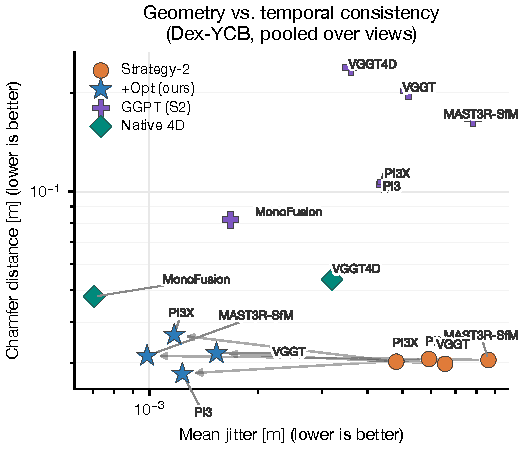
\includegraphics[width=0.85\textwidth]{figures/plotA_pareto_jitter_chamfer_v3}
\caption{Geometry vs.\ temporal consistency trade-off on DEX-YCB, pooled over view
counts. Each point represents one model--method combination. Opt-smoothed spatial
models (filled circles) cluster in the lower-left quadrant, achieving both low Chamfer
distance and low jitter simultaneously. GGPT points lie far to the right, indicating
catastrophic geometric degradation despite moderate jitter reduction. Native 4D
architectures reduce jitter but at substantially higher Chamfer than spatial models.
The lower-left corner represents the optimal operating region.}
\label{fig:pareto}
\end{figure}

\begin{figure}[t]
\centering
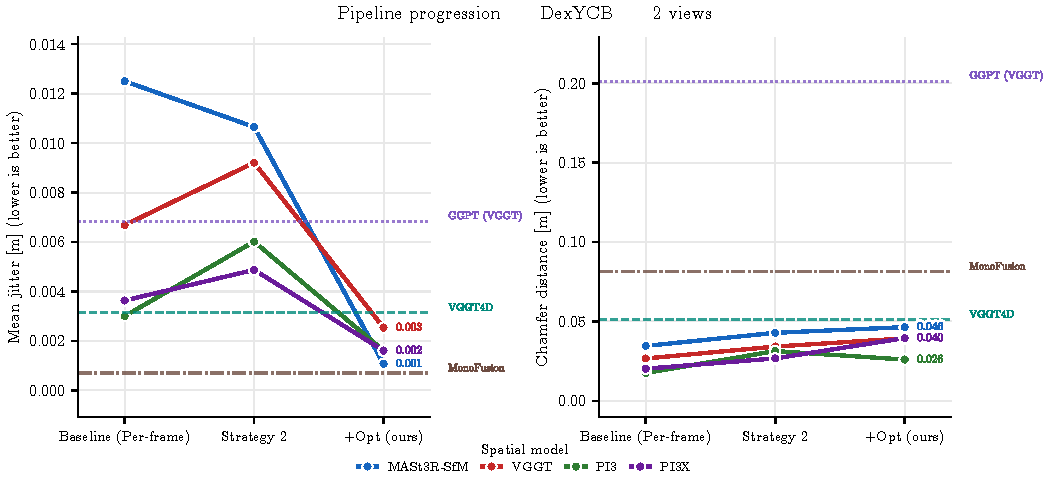
\includegraphics[width=\textwidth]{figures/plotC_pipeline_progression}
\caption{Pipeline progression on DEX-YCB at 2 views. Left panel: mean jitter across
the three pipeline stages (Baseline, Strategy-2, and Opt). Right panel: corresponding
Chamfer distance. Horizontal reference lines show VGGT4D (dashed teal) and MonoFusion
(dot-dash brown) as native 4D baselines. Opt reduces mean jitter to 0.001--0.003\,m
across all four spatial models, matching or beating VGGT4D, while Chamfer distance
remains near the Strategy-2 level for MASt3R-SfM (0.046\,m), VGGT (0.039\,m), and
PI3X (0.040\,m), and improves for PI3 (0.026\,m vs.\ 0.031\,m).}
\label{fig:pipeline_progression}
\end{figure}

\begin{figure}[t]
\centering
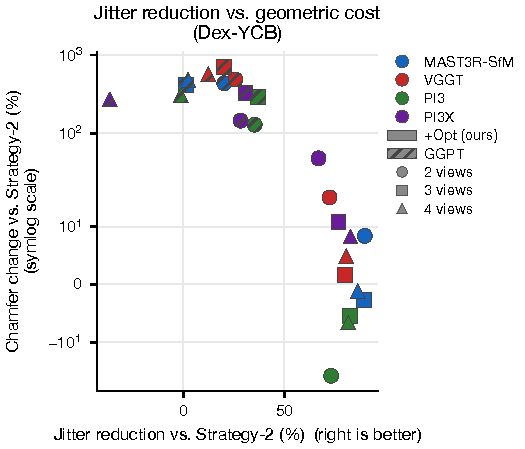
\includegraphics[width=0.85\textwidth]{figures/plotD_jitter_reduction_vs_chamfer_delta_v3}
\caption{Jitter reduction vs.\ Chamfer change relative to Strategy-2, for Opt and GGPT
across all models and view counts on DEX-YCB. The Chamfer axis uses a symmetric
log scale to accommodate the large range of GGPT degradation. Opt points cluster near
zero Chamfer change with high jitter reduction across all models and view counts. GGPT
points show consistently high positive Chamfer change (geometric degradation of
$3.8$--$8.1\times$ on DEX-YCB) with comparatively modest jitter reduction.}
\label{fig:jitter_chamfer_delta}
\end{figure}

\paragraph{Jitter reduction.}
Opt reduces mean jitter relative to Strategy-2 across all four spatial models. On
DEX-YCB at two views, MASt3R-SfM mean jitter drops from 0.011\,m to 0.001\,m
(91\,\% reduction), VGGT from 0.009\,m to 0.003\,m (67\,\%), PI3 from 0.006\,m to
0.002\,m (67\,\%), and PI3X from 0.005\,m to 0.002\,m (60\,\%). High-frequency jitter
is reduced to 0.000\,m for all four models at two views. At three and four views, the
reductions are consistent, with MASt3R-SfM and VGGT reaching 0.001\,m mean jitter in
all configurations. These jitter levels match or beat VGGT4D (0.003\,m at two and three
views) and approach MonoFusion (0.001\,m) across all view counts.

\paragraph{Geometric cost.}
The geometric impact of Opt varies across backbones. For MASt3R-SfM at three views,
Opt reduces Chamfer from 0.023\,m to 0.022\,m, a modest improvement. For VGGT, Chamfer
is unchanged at 0.028\,m at three views and increases slightly from 0.027\,m to 0.029\,m
at four views. For PI3, Chamfer improves at two views (0.031\,m to 0.026\,m) and remains
competitive at three and four views. PI3X is the exception: Opt increases Chamfer from
0.027\,m to 0.040\,m at two views (+48\,\%) and from 0.032\,m to 0.035--0.036\,m at
three and four views (+9--13\,\%). PI3X's high baseline dynamic accuracy (0.593--0.885)
is also reduced under Opt, suggesting that the static-only smoothing incidentally
affects dynamic boundary pixels, reducing the apparent dynamic accuracy. This boundary
effect is a known limitation discussed further in Chapter~\ref{c:discussion}.

\paragraph{Comparison with native 4D architectures.}
Figure~\ref{fig:pi3_case_study} illustrates the PI3+Opt vs.\ VGGT4D comparison across
view counts. At two views, PI3+Opt achieves 0.026\,m Chamfer vs.\ VGGT4D's 0.051\,m
(49\,\% lower), 0.767 static accuracy vs.\ 0.371 (107\,\% higher), and 0.002\,m mean
jitter vs.\ 0.003\,m. At three views, PI3+Opt reaches 0.033\,m Chamfer vs.\ VGGT4D's
0.041\,m, with 0.873 static accuracy vs.\ 0.625. At four views, PI3+Opt achieves
0.025\,m vs.\ VGGT4D's 0.069\,m (64\,\% lower). VGGT+Opt similarly outperforms VGGT4D
at two views on every metric: 0.039\,m vs.\ 0.051\,m Chamfer, 0.635 vs.\ 0.371 static
accuracy, and matched jitter at 0.003\,m.

\begin{figure}[t]
\centering
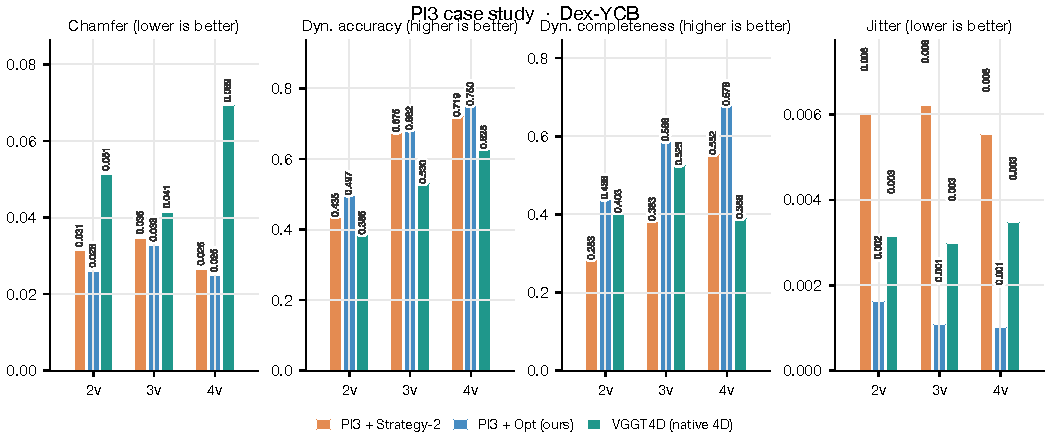
\includegraphics[width=\textwidth]{figures/plotE_pi3_case_study}
\caption{PI3 case study on DEX-YCB across view counts. PI3+Strategy-2 (blue),
PI3+Opt (orange), and VGGT4D (green) are compared on Chamfer distance, dynamic
accuracy, dynamic completeness, and mean jitter. PI3+Opt achieves lower Chamfer than
VGGT4D at all view counts while matching or improving on dynamic accuracy and
completeness. Jitter is comparable between PI3+Opt and VGGT4D at three and four views,
and lower for PI3+Opt at two views (0.002\,m vs.\ 0.003\,m). The result demonstrates
that the decoupled paradigm --- strong spatial estimation combined with targeted
temporal smoothing --- dominates the native 4D architecture on every metric at every
view count for this backbone.}
\label{fig:pi3_case_study}
\end{figure}

\paragraph{Comparison with GGPT.}
Figure~\ref{fig:jitter_chamfer_delta} shows that GGPT consistently fails to offer a
favourable trade-off. At two views, GGPT increases MASt3R-SfM's Chamfer from 0.043\,m
to 0.230\,m while reducing mean jitter from 0.011\,m to only 0.008\,m. For VGGT, GGPT
increases Chamfer from 0.034\,m to 0.201\,m with jitter reduced from 0.009\,m to
0.007\,m. Opt, by contrast, reduces MASt3R-SfM jitter from 0.011\,m to 0.001\,m while
increasing Chamfer by only 0.003\,m, and reduces VGGT jitter from 0.009\,m to 0.003\,m
while increasing Chamfer by only 0.005\,m. No configuration of GGPT Pareto-dominates
the corresponding Opt configuration on the geometry--jitter trade-off.

%% -----------------------------------------------------------------------
\section{Qualitative Analysis}
\label{sec:qualitative}

\begin{figure}[t]
\centering
% Replace with actual qualitative figure paths
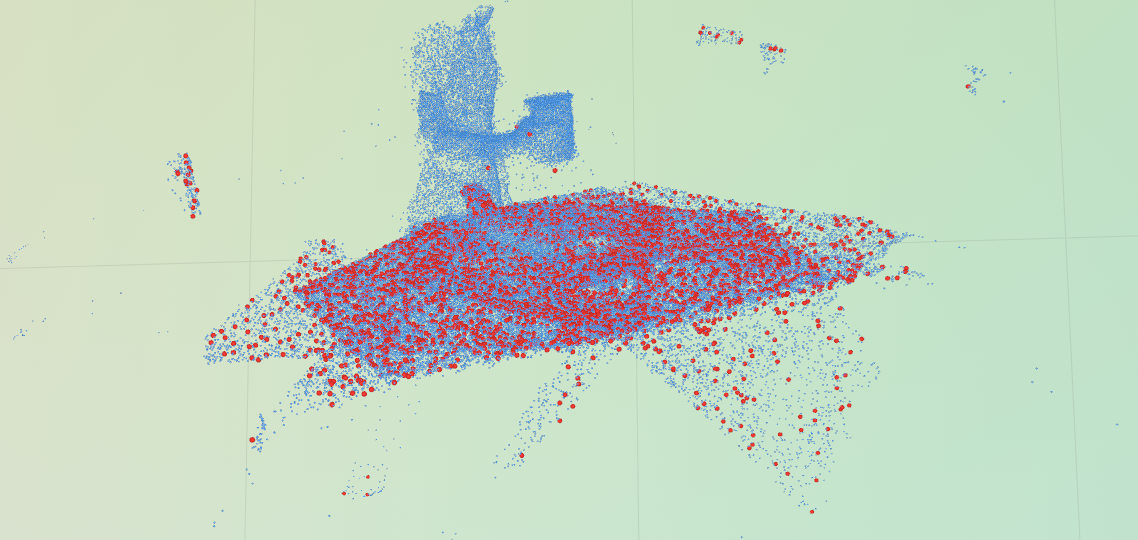
\includegraphics[width=\textwidth]{figures/qualitative_results} %TODO: Replace with actual image path
\caption{Qualitative point cloud comparisons on DEX-YCB (top two rows) and Hi4D
(bottom row). Each group shows, from left to right: Strategy-2 output, Opt-smoothed
output, VGGT4D native output, and ground truth. On DEX-YCB, Strategy-2 reconstructions
exhibit visible frame-to-frame ghosting in static background regions; Opt suppresses
these artefacts while preserving the hand and object geometry. VGGT4D reconstructions
show systematic spatial blurring of object boundaries and reduced completeness in the
manipulation region. On Hi4D, MonoFusion produces duplicated subject artefacts at two
views, where insufficient multi-view overlap causes the temporal fusion to converge to
two spatially separated copies of the same subject.}
\label{fig:qualitative}
\end{figure}

Three recurring artefact types characterise the failure modes of the evaluated
approaches. \textit{Ghosting} appears in unsmoothed spatial model outputs as
semi-transparent duplicated geometry in static regions, caused by frame-to-frame
coordinate drift in the absence of temporal alignment. Strategy-2 reduces ghosting
relative to the baseline, and Opt eliminates it in static regions entirely.
\textit{Scale drift} manifests as gradual expansion or contraction of the reconstructed
volume across the sequence, visible in MASt3R-SfM outputs at longer sequences. Opt
suppresses scale drift in static regions; the drift metric in
Table~\ref{tab:global_performance_dex_ycb} drops from 0.033\,m to 0.023\,m for
MASt3R-SfM at two views. \textit{Duplicated-subject artefacts} appear in MonoFusion
outputs at two views on Hi4D, where the temporal fusion fails to identify a consistent
depth hypothesis across the two available cameras, producing two spatially offset copies
of each subject rather than a single coherent reconstruction. These artefacts are absent
at three and four views, where sufficient overlap constrains the fusion.